\section{Deep Learning}
\subsection{Feed-Forward Neural Networks}
\textit{Function that applies linear transformation and activation functions.}

\begin{itemize}
	\item (L)inear functions $L: x\mapsto Wx + b$
	\item ($\alpha$)ctivation function: $\alpha: x \mapsto (\alpha(x_1), ..., \alpha(x_n))$
\end{itemize}

\begin{align*}
		\NN(x) 	&= \ap d (\Lp d (...\ap 2(\Lp 2((\ap 1(\Lp 1)))))) \\
				&= \ap d \circ \Lp d \hdots \ap 2 \circ \Lp 2 \circ \ap 1 \circ \Lp 1(x)
	\end{align*}

\subsubsection{Activation Functions}
\textit{Activation functions make the NN function non-linear.
}\vspace{1em}

\begin{minipage}{0.45\columnwidth}
\textbf{ReLu}: 
$$
	f(x) = \begin{cases}
		0 &\textit{for $x<0$} \\
		x &\textit{for $x\geq 0$}
	\end{cases}
$$
Danger of vanishing gradient on the left.
\end{minipage}
\begin{minipage}{0.4\columnwidth}
	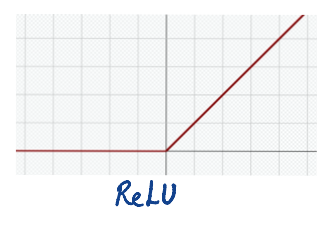
\includegraphics[width=\columnwidth]{images/10-relu}
\end{minipage}

\begin{minipage}{0.45\columnwidth}
	\textbf{Sigmoid}: 
$$
	\sigma(x) = \frac{1}{1 + \exp(-x)}
$$
Danger of vanishing gradient on both sides.
\end{minipage}
\begin{minipage}{0.4\columnwidth}
		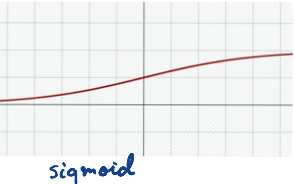
\includegraphics[width=\columnwidth]{images/10-sigmoid}
\end{minipage}

\begin{equation*}
	\sigma'(x) = 
	\begin{cases}
		\sigma(x)(1-\sigma(x)) &\textit{if dim$(x) = 1$} \\
		\sigma(x)\circ(1-\sigma(x))  &\textit{if dim$(x) > 1$}
	\end{cases}
\end{equation*}


\begin{minipage}{0.45\columnwidth}
	\textbf{Tanh}: 
$$
	\tanh(x) = \frac{2}{1 + e^{-2x}}-1
$$

Danger of vanishing gradient on both sides
\end{minipage}
\begin{minipage}{0.4\columnwidth}
		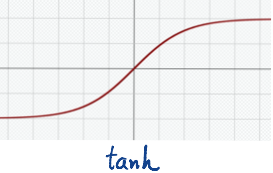
\includegraphics[width=\columnwidth]{images/10-tanh}
\end{minipage}
\vspace{1em}

\textbf{Theorem Cybenko:}\\
If $f: [0,1]^n\to\R$ is continuous, $\epsilon > 0$, then there is a neural net s.t.
\begin{enumerate}
	\item $\NN(x) = \sumim \alpha_i\sigma(w_i^Tx + b_i)$
	\item $\max_x |f(x) - \NN(x)| < \epsilon$ 
\end{enumerate}
\vspace{1em}

\textbf{Pooling Layers: } average the results from previous layer. \\
\textbf{Output Layers: }
\begin{itemize}
	\item Binary classifier: One output, $\sigma(z)$ (sigmoid)
	\item Multi-Class: Soft-max layer to get probabilities from scores: 
	\textit{"Winner takes it all"}
	$$
		y_i= \frac{\exp)\beta z_i)}{\sum_{j\leq 3}\exp(\beta z_j)t}
	$$
	
\end{itemize}
\vspace{1em}
\textbf{Training Neural Networks}
\begin{equation*}
	\min_\theta \underbrace{\sumin \L(y_i, \NN_\theta(x_i))}_{\L(\theta)}, \quad \theta = (\weight{ 1}; b^{(1)}; \weight{2}; b^{(2)}, ....),
\end{equation*}

where $\theta$ are the parameters of the neural network.This function is analytically intractable, but easy to differentiate.

\vspace{1em}
\textbf{Forward propagation: }
$$
	a^{(l)} = \sigma(Wa^{(l-1)} + b)
$$
\textbf{Back-propagation: }\\
\textit{The only purpose of back-propagation is to compute the gradients $\frac{\partial\NN}{\partial w^l}$(not optimize them, that is what optimizers are for).}
\begin{itemize}
  \item Start at the output and propagate backwards, updating weights and biases for each layer.
  \item For wach layer, back propagate the weights and biases using back-propagation algorithm: 
\end{itemize}

$$
\frac{\partial C}{\partial w^l} = \frac{\partial C}{\partial z^L} \prod_{i=L...l+1}\left(\frac{\partial z^i}{\partial a^{i-1}}\frac{\partial a^{i-1}}{\partial z^{i-1}}\right)\frac{\partial z^l}{\partial w^l},
$$
where $L$ last layer, $z$ value before activation function, $a$ value after activation function.


\begin{highlight}{Backpropagation in Multi-Layer Perceptron (Assignment 7, Ex. 1)}
\begin{minipage}{0.5\columnwidth}
	To compute the values for backpropagation, we use the chain rule.
\begin{align*}
	\frac{\partial C}{\partial \weight{l}_r} &= \frac{\partial C}{\partial\nnout{l}}\frac{\partial \nnout{l}}{\partial\weight{l}_r} \\
	\frac{\partial C}{\partial \bias{l}} &= \frac{C}{\partial\nnout{l}}\frac{\partial \nnout{l}}{\partial\bias{l}} 
\end{align*}	
For example, we got:
	$$
		\frac{\partial C}{\partial\nnout{L}} = \frac{\partial C}{\partial \activation{L}}\frac{\partial \activation{L}}{\partial\nnout{L}}
	$$

Computing and substituting all of these values will result in the iteration step of stochastic gradient descent to update the weights matrix $\weight{l}_t$ and the biase vectors $\bias{l}_t$ as
\begin{align*}
	\weight{l}_t &= \weight{l}_{t-1} - \eta \frac{\partial C}{\partial \weight{l}} \\
	\bias{l}_t &= \bias{l}_{t-1} - \eta\frac{\partial C}{\partial \bias{l}}
\end{align*}

where
$\weight{l}_t$ is the $t$-th row of the weight matrix $\weight{l}$ and $C$ is the cost of the last layers output (i.e. $\L$)
\end{minipage}
\begin{minipage}{0.5\columnwidth}
	\begin{flushright}
		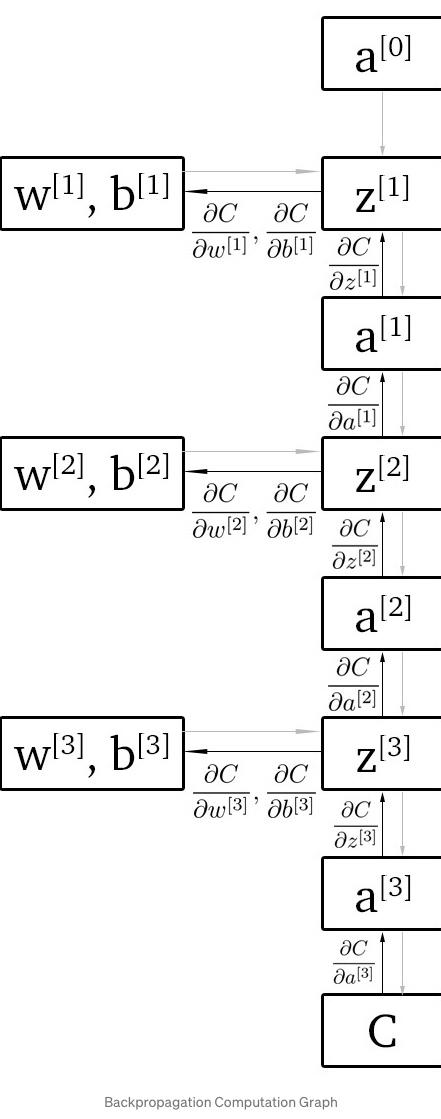
\includegraphics[width=0.8\columnwidth]{images/10-backpropagation}
	\end{flushright}
\end{minipage}
\end{highlight}

\subsubsection{Gradient Descent}
\begin{algorithm}[H]  
	$k\gets 0$ \\
	$\weight{k}_r \gets$ Unif$([-\sqrt{\frac{1}{n}}, \sqrt{\frac{1}{n}}])$ for $\l \leq d, r\leq$\#rows $W^{(l)}$ \\
   \DoUntil{\textit{difference between test-cost and train-cost starts increasing}}
   {
      $w^{(k+1)} \gets w^{(k)} - \eta(k)\nabla_{\weight l_r} \L(\theta)$ for $\l \leq d, \forall r $
      
      $k\gets k+1$ 
  	}
  \caption{General Form of Gradient Descent}
\end{algorithm}

%\begin{highlight}{How to compute $\nabla_{\weight{l}_r} \L(\theta)$}
%	\begin{enumerate}
%		\item Jacobian matrix: $\left(\frac{\partial F_i}{\partial w_j} \right)_{\substack{i\leq n\\ j\leq m}} : \R^m\to\R^{n\times m}$
%		\item Use the chain rule
%	\end{enumerate}
%	\todo[inline]{TODO: How is it done + example!}
%\end{highlight}

\begin{algorithm}[H]  
	$k\gets 0$ \\
	$\weight{k}_r \gets$ Unif$([-\sqrt{\frac{1}{n}}, \sqrt{\frac{1}{n}}])$ for $\l \leq d, r\leq$\#rows $W^{(l)}$ \\
   \RepeatUntil{\textit{...}}
   {
      do fwd and back propagation to compute $\frac{\partial \NN}{\partial\weight{l}_r} \vert_{\theta, x_i} $ for each $l,r,i\leq n$ \\
      $\frac{\partial\L}{\weight{l}_r} =\sumin \frac{\partial \L(y_i, \NN_\theta(x_i))}{\partial \weight{l}_r}$ \\
      $\weight{l}_r \gets \weight{l}_r - \eta(k) \frac{\partial \L}{\partial\weight{l}_r}$
  	}
  \caption{Gradient Descent}
\end{algorithm}

\begin{algorithm}[H]  
	$k\gets 0$ \\
	$\weight{k}_r \gets$ Unif$([-\sqrt{\frac{1}{n}}, \sqrt{\frac{1}{n}}])$ for $\l \leq d, r\leq$\#rows $W^{(l)}$ \\
   \RepeatUntil{\textit{...}}
   {
      do fwd and back propagation to compute $\frac{\partial \NN}{\partial\weight{l}_r} \vert_{\theta, x_i} $ for each $l,r,$ {\color{imp}$i\in S$, where $S$ is a sample from $\{1...n\}$} \\ 

      $\frac{\partial\L}{\weight{l}_r} =\sumin \frac{\partial \L(y_i, \NN_\theta(x_i))}{\partial \weight{l}_r} {\color{imp}\approx \sum_{i\in S}\frac{\partial \L(y_i, \NN_\theta(x_i))}{\partial \weight{l}_r}}$ \\
      $\weight{l}_r \gets \weight{l}_r - \eta(k) \frac{\partial \L}{\partial\weight{l}_r}$
  	}
  \caption{Mini-Batch (stochastic) Gradient Descent}
\end{algorithm}

\textbf{SGD as stochastic optimization}
$$
	\min_\theta \sumin \L(y_i, \NN_\theta(x_i))
$$
\begin{align*}
	\iff 0 	&= \sumin\nabla_\theta\L(y_i, \NN_\theta(x_i)) \\
			&= \hat\E_{x,y}[\nabla_\theta\L(Y, \NN_\theta(x)] \\
			&\approx \E_{x,y}[\nabla_\theta\L(Y, \NN_\theta(x)] \\
			&= \E_{x,y}[\nabla_\theta f(X,Y; \theta)] \\
			\Leftarrow \E_{x,y}[\nabla_\theta f(X,Y; \theta)] &= 0
\end{align*}

\textbf{Comparison Gradient Descent}

\begin{center}
	\begin{tabular}{ p{0.45\columnwidth} | p{0.45\columnwidth} } 
		\textbf{Batch GD} & \textbf{Mini-batch / stochastic GD}\\\hline
		\begin{itemize}[leftmargin=*]
			\item More precise gradient
			\item Larger generalization error
		\end{itemize}
		&
		\begin{itemize}[leftmargin=*]
			\item Can handle large training sets
			\item Faster improvements
			\item Escapes local minimum
		\end{itemize}
	\end{tabular}
\end{center}

\subsubsection{Robbins-Monro algorithm}
\textit{Methodology for solving a root finding problem (of the expected value $\E$). Provides convergence guarantee for SGD (see below).}

\begin{algorithm}[H]  
	\SetKwInOut{Input}{input}
	\SetKwInOut{Output}{output}

	\Input{Learning rate function $\eta$ \\ sample $z_1, z_2, ...$}
	\Output{$\theta$ s.t. $\E_Z[f(Z;\theta)] = 0$}
	$\theta^{(0)} \gets \$$ \\
	\For{$k = 0...$}{
		$\theta^{(k)} \gets \theta^{(k-1)} - \eta(k) f(z_k; \theta^{(k-1)})$
  	}
  \caption{Robbin-Monro algorithm}
\end{algorithm}

\textbf{Convergence: } If $\E_Z[f(Z;\theta)]$ satisfies some regularity conditions, $\eta(k) \geq 0, \sum_k \eta(k) = \infty, \sum_k \eta^2(k) < \infty$, then 

\begin{align*}
	\E[(\theta^{(k)} - \theta^*)^2] &\xrightarrow{k\to\infty} 0 \\
	P[\theta^{(k)} = \theta^*)] &\xrightarrow{k\to\infty} 1
\end{align*}


\begin{minipage}{0.6\columnwidth}
\textbf{Regularity Conditions: }\\
	$\E_Z[f(Z;\theta^*)] < \E_Z[f(Z;\theta)], \forall \theta > \theta^*$ \\
	$\E_Z[f(Z;\theta^*)] > \E_Z[f(Z;\theta)], \forall \theta < \theta^*$ \\
	There are other formulations (see Slides p.32)
\end{minipage}
\begin{minipage}{0.3\columnwidth}
	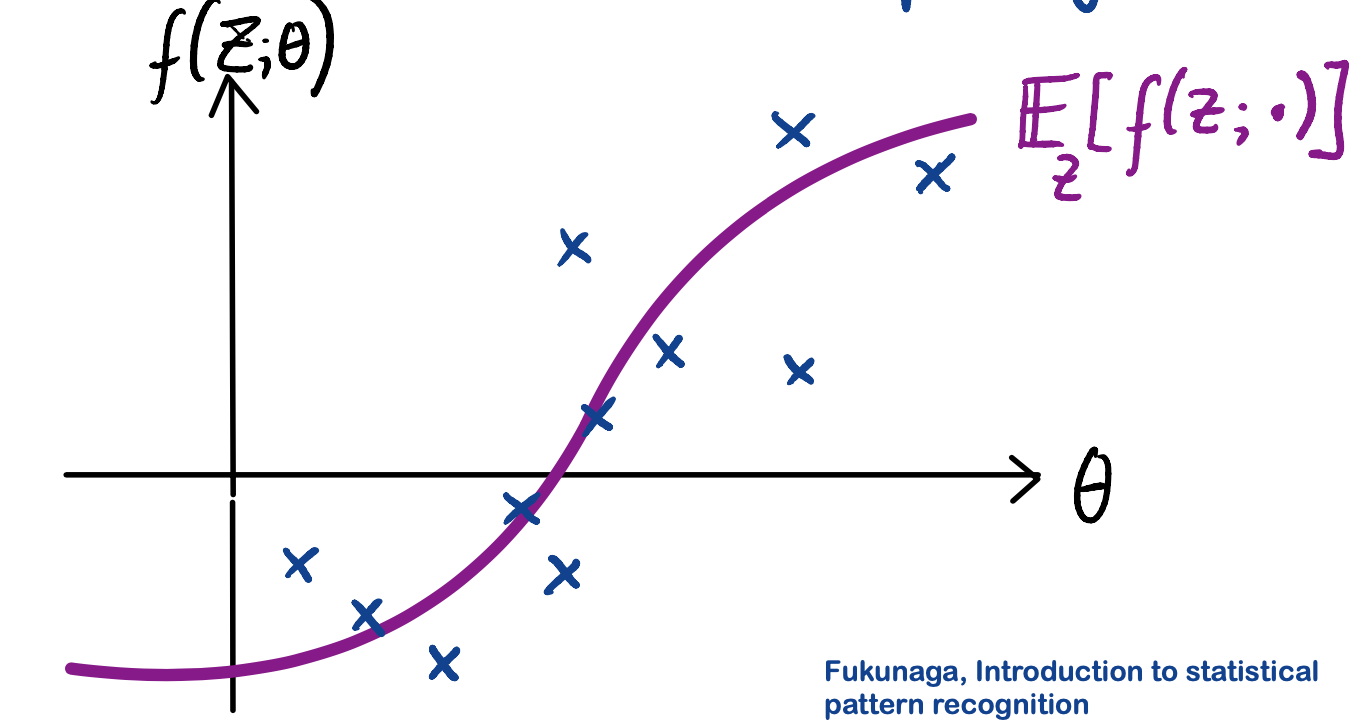
\includegraphics[width=\columnwidth]{images/10-robbin-monro}
\end{minipage}






